%==============================================================================
% UniVR Chatbot - Project Documentation
% A RAG-Powered AI Assistant for University of Verona
%==============================================================================

\documentclass[12pt,a4paper]{article}

%------------------------------------------------------------------------------
% Packages
%------------------------------------------------------------------------------
\usepackage[utf8]{inputenc}
\usepackage[T1]{fontenc}
\usepackage{graphicx}
\usepackage{geometry}
\usepackage{hyperref}
\usepackage{xcolor}
\usepackage{tikz}
\usepackage{tcolorbox}
\usepackage{enumitem}
\usepackage{booktabs}
\usepackage{fancyhdr}
\usepackage{titlesec}
\usepackage{float}

% TikZ libraries
\usetikzlibrary{shapes.geometric, arrows.meta, positioning, fit, backgrounds, calc}

%------------------------------------------------------------------------------
% Page Setup
%------------------------------------------------------------------------------
\geometry{
    left=2.5cm,
    right=2.5cm,
    top=3cm,
    bottom=3cm
}

% Colors
\definecolor{univrred}{RGB}{187, 0, 0}
\definecolor{univrbg}{RGB}{245, 245, 250}
\definecolor{darkblue}{RGB}{30, 60, 120}
\definecolor{lightblue}{RGB}{200, 220, 255}

% Header/Footer
\pagestyle{fancy}
\fancyhf{}
\fancyhead[L]{\footnotesize UniVR Chatbot Documentation}
\fancyhead[R]{\footnotesize \thepage}
\renewcommand{\headrulewidth}{0.4pt}

% Section formatting
\titleformat{\section}
    {\Large\bfseries\color{univrred}}
    {\thesection}{1em}{}[\titlerule]
\titleformat{\subsection}
    {\large\bfseries\color{darkblue}}
    {\thesubsection}{1em}{}

% Hyperref setup
\hypersetup{
    colorlinks=true,
    linkcolor=darkblue,
    urlcolor=univrred,
    citecolor=darkblue
}

%------------------------------------------------------------------------------
% TikZ Styles
%------------------------------------------------------------------------------
\tikzstyle{component} = [
    rectangle, 
    rounded corners=8pt, 
    minimum width=3cm, 
    minimum height=1.2cm, 
    text centered, 
    draw=darkblue, 
    fill=lightblue,
    font=\small\bfseries
]
\tikzstyle{database} = [
    cylinder, 
    shape border rotate=90, 
    aspect=0.25, 
    minimum width=2.5cm, 
    minimum height=1.5cm, 
    draw=darkblue, 
    fill=lightblue!60
]
\tikzstyle{user} = [
    circle, 
    minimum size=1.2cm, 
    draw=univrred, 
    fill=univrred!15,
    font=\small\bfseries
]
\tikzstyle{arrow} = [
    thick, 
    ->, 
    >=Stealth, 
    color=darkblue
]
\tikzstyle{dashedarrow} = [
    thick, 
    dashed, 
    ->, 
    >=Stealth, 
    color=gray
]

%==============================================================================
% Document Begin
%==============================================================================
\begin{document}

%------------------------------------------------------------------------------
% Title Page
%------------------------------------------------------------------------------
\begin{titlepage}
    \centering
    \vspace*{2cm}
    
    {\Huge\bfseries\color{univrred} UniVR Chatbot\par}
    \vspace{0.5cm}
    {\Large A RAG-Powered AI Assistant\par}
    {\Large for the University of Verona\par}
    
    \vspace{2cm}
    
    % Simple illustration
    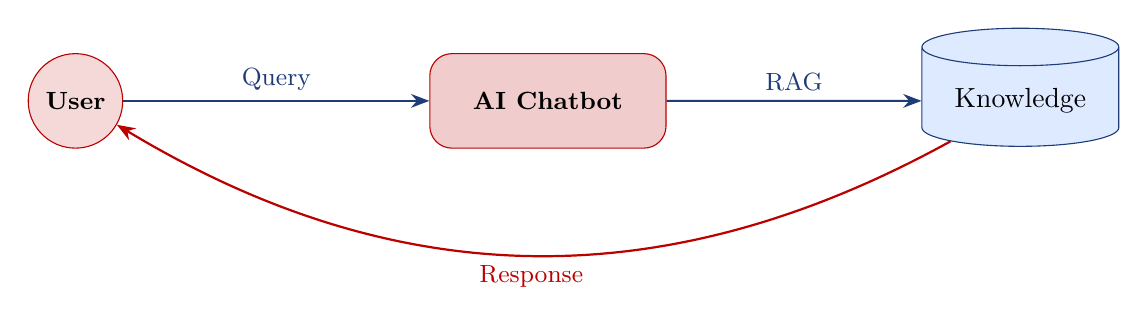
\begin{tikzpicture}[scale=1.2]
        % User icon
        \node[user] (user) at (0,0) {User};
        
        % Chatbot icon
        \node[component, fill=univrred!20, draw=univrred] (bot) at (5,0) {AI Chatbot};
        
        % Knowledge base
        \node[database] (kb) at (10,0) {Knowledge};
        
        % Arrows
        \draw[arrow] (user) -- node[above]{\small Query} (bot);
        \draw[arrow] (bot) -- node[above]{\small RAG} (kb);
        \draw[arrow, color=univrred] (kb) to[bend left=30] node[below]{\small Response} (user);
    \end{tikzpicture}
    
    \vspace{3cm}
    
    {\large\textbf{Project Documentation}\par}
    \vspace{0.5cm}
    {\large Version 1.0\par}
    
    \vfill
    
    {\normalsize Università degli Studi di Verona\par}
    {\normalsize \today\par}
\end{titlepage}

%------------------------------------------------------------------------------
% Table of Contents
%------------------------------------------------------------------------------
\tableofcontents
\newpage

%==============================================================================
% Section 1: Project Overview
%==============================================================================
\section{Project Overview}

This short document summarizes the \textbf{RAG-based generic chatbot} prototype I implemented.
The goal of the prototype is not a finished UniVR product, but a reusable
kick-start platform that can support \emph{any} domain by connecting
domain documents to a Retrieval-Augmented Generation (RAG) pipeline.

\begin{tcolorbox}[colback=univrbg, colframe=univrred, title=\textbf{What I Implemented}]
    \begin{itemize}[noitemsep]
        \item A \textbf{backend} in FastAPI that exposes chat and admin APIs
        \item A \textbf{frontend} in Next.js that provides a simple chat UI and domain selector
        \item A \textbf{multi-domain RAG layer} built on Google Gemini File Search and File Stores
    \end{itemize}
\end{tcolorbox}

Instead of hard-coding one university use case, the system lets us create
multiple independent domains (e.g.\ ``Scholarships'', ``Admissions'', ``International'')
and query each domain using the same generic chatbot logic.

%==============================================================================
% Section 2: High-Level Architecture
%==============================================================================
\section{High-Level Architecture}

The system follows a simple three-layer architecture:

\begin{itemize}
    \item \textbf{Frontend (Next.js)} --- renders the chat UI, lets the user choose a domain,
          and sends chat requests to the backend.
    \item \textbf{Backend (FastAPI)} --- exposes REST endpoints, selects the right domain,
          orchestrates calls to Gemini and File Search, and returns grounded answers.
    \item \textbf{AI + Knowledge (Gemini + File Stores)} --- stores uploaded PDFs per domain,
          performs retrieval, and powers the RAG responses.
\end{itemize}

\begin{figure}[H]
    \centering
    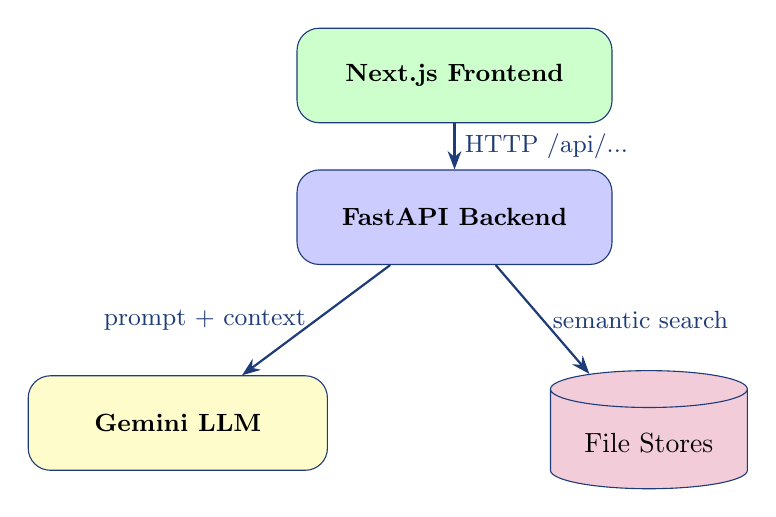
\begin{tikzpicture}[node distance=1.8cm]
        \node[component, fill=green!20, minimum width=4cm] (fe) {Next.js Frontend};
        \node[component, fill=blue!20, minimum width=4cm, below of=fe] (be) {FastAPI Backend};
        \node[component, fill=yellow!20, minimum width=3.8cm, below left=1.4cm and -0.4cm of be] (gemini) {Gemini LLM};
        \node[database, fill=purple!20, below right=1.4cm and -0.4cm of be] (stores) {File Stores};

        \draw[arrow] (fe) -- node[right]{\small HTTP /api/...} (be);
        \draw[arrow] (be) -- node[left]{\small prompt + context} (gemini);
        \draw[arrow] (be) -- node[right]{\small semantic search} (stores);
    \end{tikzpicture}
    \caption{High-level architecture of the generic RAG chatbot}
\end{figure}

%==============================================================================
% Section 3: RAG Flow Per Domain
%==============================================================================
\section{RAG Flow Per Domain}

Each domain is backed by a separate File Store. The same flow is reused for
any domain:

\begin{enumerate}
    \item \textbf{Domain selection}: the frontend calls \texttt{GET /api/domains} and shows
          the available domains returned by the backend.
    \item \textbf{User question}: the user selects a domain and sends a question via
          \texttt{POST /api/chat} with the domain id.
    \item \textbf{Retrieval}: the backend uses the configured File Store for that domain
          to retrieve the most relevant document chunks using Gemini File Search.
    \item \textbf{Grounded generation}: the backend calls Gemini with the user question
          plus retrieved passages as context (RAG).
    \item \textbf{Response}: the backend returns the answer and the sources; the frontend
          renders them in the chat.
\end{enumerate}

\begin{figure}[H]
    \centering
    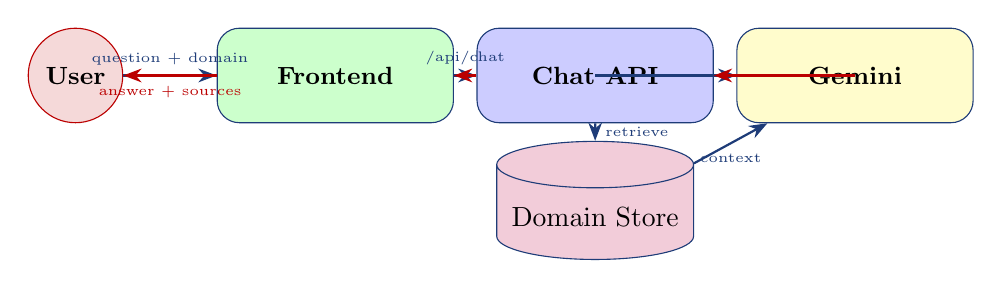
\begin{tikzpicture}[node distance=1.5cm]
        \node[user] (user) {User};
        \node[component, fill=green!20, right of=user, xshift=1.8cm] (fe) {Frontend};
        \node[component, fill=blue!20, right of=fe, xshift=1.8cm] (api) {Chat API};
        \node[database, fill=purple!20, below of=api, yshift=-0.3cm] (store) {Domain Store};
        \node[component, fill=yellow!20, right of=api, xshift=1.8cm] (llm) {Gemini};

        \draw[arrow] (user) -- node[above]{\tiny question + domain} (fe);
        \draw[arrow] (fe) -- node[above]{\tiny /api/chat} (api);
        \draw[arrow] (api) -- node[right]{\tiny retrieve} (store);
        \draw[arrow] (store) -- node[below]{\tiny context} (llm);
        \draw[arrow] (api) |- (llm);
        \draw[arrow, color=univrred] (llm) |- (api);
        \draw[arrow, color=univrred] (api) -- (fe);
        \draw[arrow, color=univrred] (fe) -- node[below]{\tiny answer + sources} (user);
    \end{tikzpicture}
    \caption{RAG flow for a single selected domain}
\end{figure}

%==============================================================================
% Section 4: Implementation Summary
%==============================================================================
\section{Implementation Summary}

\subsection{Backend (FastAPI)}

\begin{itemize}
    \item Implemented main application in \texttt{app.main} with CORS, static files, and a health check.
    \item Added \textbf{chat API} endpoints under \texttt{/api} for:
          listing domains, sending chat messages, and returning suggestions.
    \item Implemented an \textbf{agent layer} that wraps Gemini:
          given a domain id and question, it runs retrieval on the matching File Store
          and builds a grounded prompt for the model.
\end{itemize}

\subsection{Frontend (Next.js)}

\begin{itemize}
    \item Single-page app with:
          a domain selection view and a chat interface view.
    \item Uses a configurable \texttt{NEXT\_PUBLIC\_API\_URL} so it can talk to any deployed backend
          (local or on Render).
    \item Renders the model answer and shows which documents were used as sources.
\end{itemize}

\subsection{Domain Management}

\begin{itemize}
    \item Domains are identified by a prefix and mapped to separate File Stores.
    \item Admin endpoints allow uploading new PDFs to a domain; the content is indexed
          by Gemini File Search.
    \item The same generic chat endpoint works for all domains, only the store id changes.
\end{itemize}

%==============================================================================
% Section 5: Example Use and Next Steps
%==============================================================================
\section{Example Use and Next Steps}

\subsection{Example: Scholarship Domain}

As a concrete example, I created a ``Scholarships'' domain and uploaded official
PDF calls for applications. Students can ask questions such as:

\begin{itemize}
    \item ``What are the main eligibility requirements for this scholarship?''
    \item ``What is the application deadline and where do I submit the form?''
\end{itemize}

The chatbot answers using the text retrieved from the uploaded PDFs, and the
frontend shows which file and section were used.

\subsection{Next Steps (After This Prototype)}

\begin{itemize}
    \item Add authentication and simple admin UI for uploading documents and managing domains.
    \item Improve prompt design and answer formatting for long, legal-style PDF documents.
    \item Deploy backend (Render) and frontend (Vercel) for stable public access.
    \item Evaluate quality with real student questions and refine domains and documents.
\end{itemize}

\section{Conclusion}

This prototype demonstrates a \textbf{generic, multi-domain RAG chatbot} that can be reused
for different university domains by simply uploading new documents and creating new stores.
The focus of this work is on the integration of FastAPI, Next.js and Gemini File Search
into a clean, extensible architecture that can serve as a starting point for a more
complete UniVR chatbot in the future.

%==============================================================================
% End Document
%==============================================================================
\end{document}
